\subsection{Proposed Timeline}
\todo[inline]{A Gantt chart, perhaps with critical tasks highlighted, to be detailed below}
Figure \ref{fig::gantt_chart} shows my proposed timeline to complete my thesis work. Most work is to be completed during the first semester of next year, though I have organised to get as much research complete over the summer break so I can use my time more appropriately during semester. The red bars show an alternate pathway to a working solution, if the \gls{pcie} digitizer or MATLAB is unable to perform the required task.
\begin{figure}[htbp!]
	\centering
	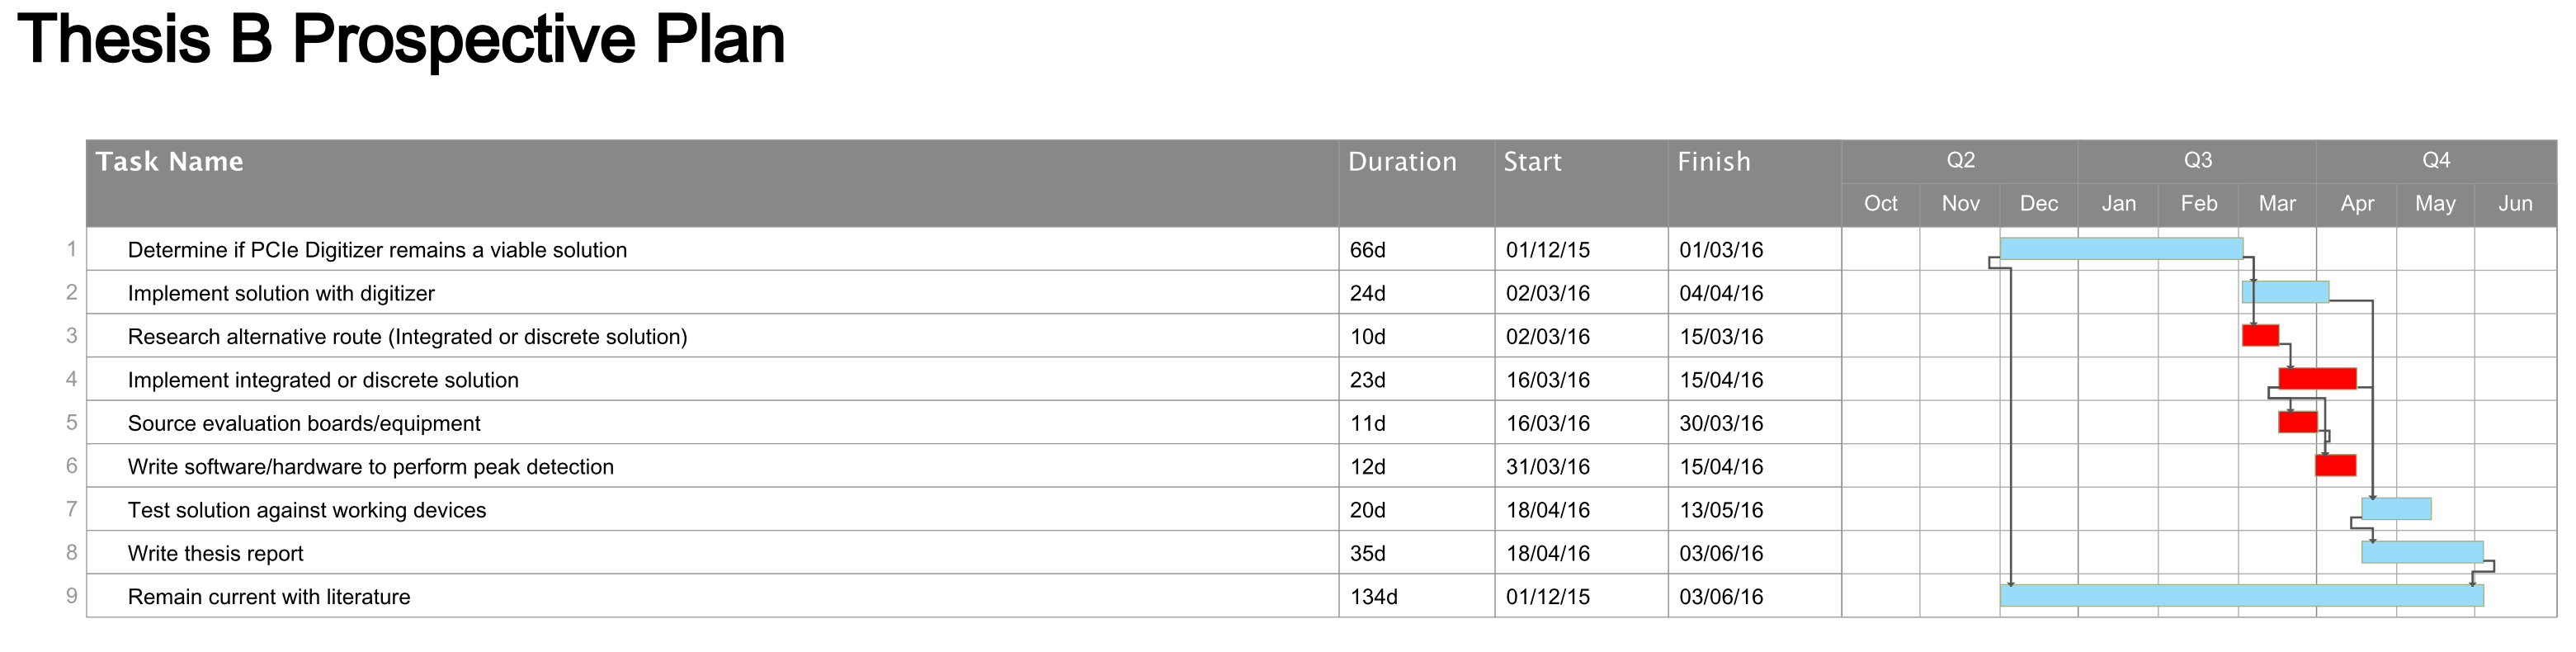
\includegraphics[width=\textwidth]{gantt_chart}
	\caption{Gantt Chart}
	\label{fig::gantt_chart}
\end{figure}

\subsection{Description of Work}

The following lists are the final avenues available in utilizing the \gls{pcie} digitizer and MATLAB solution.
\begin{itemize}
	\item Software Triggering
	\item Continuous \gls{dma}
	\item Manual external triggering
\end{itemize}
By the beginning of semester I will be able to confirm or deny if any of these solutions will work. A brief detail of each method

\todo[inline]{Details about what the particulars of work to be done are}

\todo[inline]{Talk about further options with PCIe digitizer, manual triggering in MATLAB, manual external triggering from an ARB (software controlled), or continuous DMA}